\documentclass[12pt]{report}

\usepackage{amsmath}
\usepackage{pgfplots}
\usepgfplotslibrary{units}
\usepackage[russian]{babel}
\usepackage{filecontents}
\usepackage{titlesec, blindtext, color}
\usepackage{listings}

\usepackage{titlesec, blindtext, color} 
\definecolor{gray75}{gray}{0.75} 
\newcommand{\hsp}{\hspace{20pt}} 

\usepackage{geometry}
\geometry{top=0.5cm}


\lstset{ 
language=haskell,                 
basicstyle=\small\sffamily, 
numbers=left,              
numberstyle=\tiny,        
stepnumber=1,              
numbersep=5pt,             
showspaces=false,          
showstringspaces=false,   
showtabs=false,             
frame=single,            
tabsize=2,                
captionpos=t,              
breaklines=true,           
breakatwhitespace=false, 
escapeinside={\#*}{*)}   
}

\titleformat{\chapter}[hang]{\Huge\bfseries}{\thechapter\hsp\textcolor{gray75}{|}\hsp}{0pt}{\Huge\bfseries}

\begin{filecontents}{bSort_times_proc.dat}
1000 0.01937
1100 0.01962
1200 0.02371
1300 0.02616
1400 0.02823
1500 0.03296
1600 0.03725
1700 0.04761
1800 0.05449
1900 0.06122
2000 0.06756
\end{filecontents}

\begin{filecontents}{bSort_timesF_proc.dat}
1000 0.01922
1100 0.02103
1200 0.02419
1300 0.02832
1400 0.03067
1500 0.03516
1600 0.03759
1700 0.0454
1800 0.05219
1900 0.06051
2000 0.06591
\end{filecontents}

\begin{filecontents}{bSort_timesR_proc.dat}
1000 0.02464
1100 0.02384
1200 0.03504
1300 0.03601
1400 0.04114
1500 0.04539
1600 0.05999
1700 0.07741
1800 0.07027
1900 0.08
2000 0.08919
\end{filecontents}

\begin{filecontents}{inSort_times_proc.dat}
1000 0.00029
1100 0.00019
1200 0.00026
1300 0.00015
1400 0.00033
1500 0.00019
1600 0.00025
1700 0.00042
1800 0.00035
1900 0.00028
2000 0.00029
\end{filecontents}

\begin{filecontents}{inSort_timesF_proc.dat}
1000 2e-05
1100 0.00019
1200 7e-05
1300 9e-05
1400 0.00023
1500 6e-05
1600 5e-05
1700 0.0001
1800 0.0002
1900 6e-05
2000 9e-05
\end{filecontents}

\begin{filecontents}{inSort_timesR_proc.dat}
1000 8e-05
1100 4e-05
1200 9e-05
1300 5e-05
1400 9e-05
1500 0.00029
1600 0.00012
1700 0.00016
1800 9e-05
1900 0.00016
2000 0.00015
\end{filecontents}

\begin{filecontents}{qSort_times_proc.dat}
1000 0.00065
1100 0.00064
1200 0.00042
1300 0.00067
1400 0.00068
1500 0.00095
1600 0.00071
1700 0.00143
1800 0.00133
1900 0.00145
2000 0.0022
\end{filecontents}

\begin{filecontents}{qSort_timesF_proc.dat}
1000 0.00026
1100 0.00033
1200 0.00028
1300 0.00024
1400 0.00031
1500 0.00034
1600 0.00031
1700 0.00033
1800 0.00034
1900 0.00033
2000 0.00037
\end{filecontents}

\begin{filecontents}{qSort_timesR_proc.dat}
1000 0.05463
1100 0.05893
1200 0.08216
1300 0.09325
1400 0.10566
1500 0.11752
1600 0.14982
1700 0.18477
1800 0.17601
1900 0.19965
2000 0.22478
\end{filecontents}


\begin{document}

\begin{titlepage}
	\centering
	{\scshape\LARGE МГТУ им. Баумана \par}
	\vspace{3cm}
	{\scshape\Large Лабораторная работа №3\par}
	\vspace{0.5cm}	
	{\scshape\Large По курсу: "Анализ алгоритмов"\par}
	\vspace{1.5cm}
	{\huge\bfseries Сортировки\par}
	\vspace{2cm}
	\Large Работу выполнил: Подвашецкий Дмитрий, ИУ7-54Б\par
	\vspace{0.5cm}
	\LargeПреподаватели:  Волкова Л.Л., Строганов Ю.В.\par

	\vfill
	\large \textit {Москва, 2019} \par
\end{titlepage}

\tableofcontents

\newpage
\chapter*{Введение}
\addcontentsline{toc}{chapter}{Введение}

	\textbf{Алгоритм сортировки} - это алгоритм, позволяющий упорядочить элементы в некотором списке. Сортировки - это основа, которую учат все, кто так или иначе хочет заниматься чем-либо связанным с программированием. 

	За все время было создано огромное множество различных алгоритмов сортировки, каждая из которых обладает какими-либо особенности. В данной лабораторной работе я постраюсь это продемонстрировать.

	\textbf{Задачами} данной лабораторной работы являются:
\begin{enumerate}
	\item выбор и изучение трех алгоритмов сортировки;
	\item реализация выбранных алгоритмов;
	\item теоретический анализ сложности;
	\item эксперементальное подтверждение различий во временной эффективности алгоритмов;
	\item описание и обоснование полученных результатов в отчете о выполненной лабораторной
работе, выполненного как расчётно-пояснительная записка к работе.
\end{enumerate}

\chapter{Аналитическая часть}

	Для рассмотрения в этой лабораторной работе мною были выбраны алгоритмы:
\begin{enumerate}
	\item быстрой сортировки;
	\item сортироки пузырьком;
	\item сортировки вставками.
\end{enumerate}

\section{Быстрая сортировка}
	

	Суть данного алгоритма заключается в выборе некоторого опортного элемента (обычно выбирают либо последний, либо средний) и дальнейшем разбиении списка на два подсписка: все элементы меньше опортного и все те, что больше опорного. Далее для каждого из двух подсписков рекурсивно применяется тот же алгоритм сортировки.

Обозначим: 

{ qSort(list) - применение алгоритма быстрой сортировки к некоторому списку list.  }

{$ list = l_{0}, l_{1}, ... , l_{n}  $}

{$ listL =  l_{i} :  l_{i} <=  l_{0}, i = 1..n  $}

{$ listR = l_{i} :  l_{i} >  l_{0}, i = 1..n  $}


Тогда алгоритм быстрой сортировки можно записать как:
\begin{equation}
	qSort(list) = qSort(listL) + l_{0} + qSort(listR)
\end{equation}

\section{Сортировка пузырльком}

	Данный алгоритм заключается в проходе списка слева направо до конца. Если текущий элемент больше следующего, то необходимо поменять их местами (для сортировки по возрастанию). Заметим, что после, этот процесс необходимо повторять до тех пор, пока массив не будет отсортирован. В случае если алгоритм никак не модифицирован, то необходимо повторить кол-во раз, равного длине массива.

\section{Сортировка вставками}

	Суть этого алогоритма аключается в том что, на каждом шаге алгоритма мы берем один из элементов массива, находим позицию для вставки и вставляем. Стоит отметить что массив из 1-го элемента считается отсортированным. [1] В ходе работы данного алгоритма, при обратоке i-го элемента можно быть уверенным в том, что левая часть является полностью остортированной.
	
\section*{Вывод}
\addcontentsline{toc}{chapter}{Вывод}

	В данном разделе мною было рассмотрены и вкратце описаны рассматриваемые мною алгоритмы.


\chapter{Конструкторский раздел}
\section{Схемы алгоритмов и их анализ}

\subsection{Быстрая сортировка}


\begin{center}
		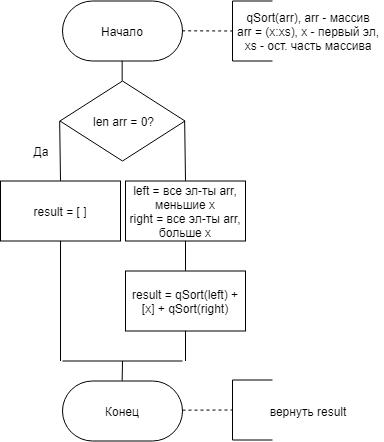
\includegraphics[scale=0.6]{qSort.png}
		
			Рис 2. Схема алгоритма быстрой сортировки.
\end{center}

\begin{center}
	\textbf{Лучший случай:}
\end{center}
	Лучший случай достигается тогда, когда при каждом вызове функции массив делится пополам (+- 1 элемент).
Рекурсия завершается если в обрабатываемом массиве остался только 1 элемент.
В таком случае, массив делится на {$N/2$} и {$N/2$}, следовательно чтобы найти максимальную глубину рекурсии необходимо найти i из уравнения {$N/2^i = 1$}. i = {$log_{2}(N)$}, из чего следует, что трудоемкость алгоритма равна: {$N*log_{2}(N)$}

\begin{center}
	\textbf{Худший случай:}
\end{center}
	В худшем случае каждое разделение дает два подмассива длины 1 и N-1. При выборе опорного элемента первым или последним, такой эффект даст полностью отсортированный массив.
	Максимальная глубина рекурсии в таком случае равна N, из чего следует, что трудоемкость алгоритма равно: {$O(N^2)$}

\subsection{Сортировка пузырьком}


\begin{minipage}{0.5\textwidth}
  \begin{flushleft}
	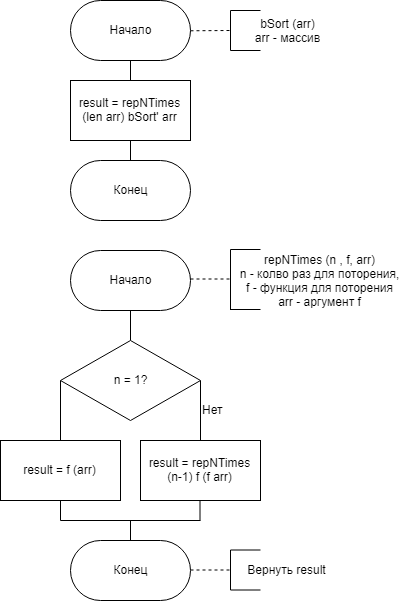
\includegraphics[scale=0.6]{bSort.png}
  \end{flushleft}
\end{minipage}
\hfill
\begin{minipage}{0.5\textwidth}
  \begin{flushright}
	\begin{center}
	bSort - это функция 'надстройка', едиснтвенная её задача - вызов функции repNTimes, следовательно
	\begin{equation}
	F_{bSort} = F_{repNTimes}
	\end{equation}
	~\\
	~\\
	~\\
	~\\
	~\\
	~\\
	~\\
	~\\
	~\\
	Максимальная глубина рекурсии функции repNTimes = N, что равно длине массива
	\begin{equation}
	F_{repNTimes} = N(2 + F_{bSort'}) - 1
	\end{equation}
	\end{center}
  \end{flushright}
\end{minipage}

\begin{minipage}{0.5\textwidth}
  \begin{flushleft}
	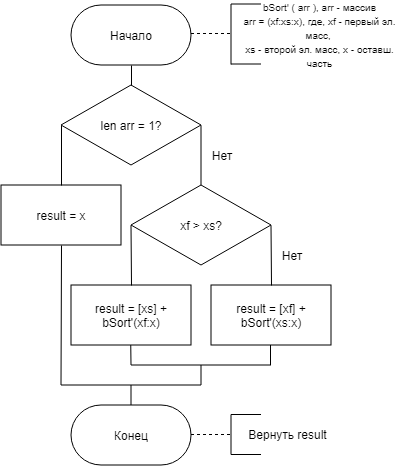
\includegraphics[scale=0.6]{bSort2.png}

	Рис 2. Схема алгоритма сортировки пузырьком.
  \end{flushleft}
\end{minipage}
\hfill
\begin{minipage}{0.5\textwidth}
  \begin{flushright}
	\begin{center}
		Максимальная глубина рекурсии bSort' так же равна N
		\begin{equation}
		F_{bSort'} = 3N - 1
		\end{equation}
	\end{center}
  \end{flushright}
\end{minipage}

\begin{center}
\textbf{Анализ трудоемкости:}
\begin{equation}
	F_{bSort} = F_{repNTimes} = N(2 + F_{bSort'}) - 1 = N(2 + 3N - 1) - 1 = N + 3N^2 - 1
\end{equation}

Для данной реализации алгоритма сортировки пузрьком, нет различий в трудоемкости при обратке обратно отсортированного массива, прямого или случайного.

Общая сложность алгоритма для всех случаев: {$O(N^2)$}
\end{center}

\subsection{Сортировка вставками}

\begin{center}
	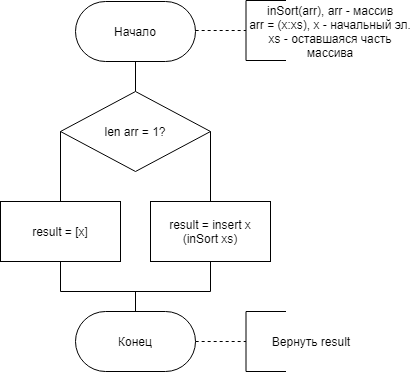
\includegraphics[scale=0.6]{inSort1.png}
	
	
	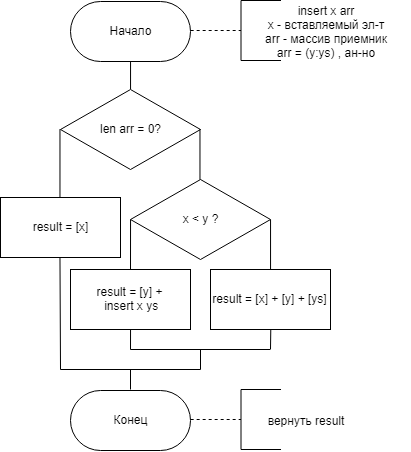
\includegraphics[scale=0.6]{inSort2.png}
	
	Рис 3. Схема алгоритма сортировки вставками.
\end{center}

\begin{center}
	\textbf{Анализ трудоемкости:}
\end{center}
Согласно [3]:

\textbf{Лучший случай} - {$O(N)$}

\textbf{Худший случай} - {$O(N^2)$}

\section*{Вывод}
\addcontentsline{toc}{chapter}{Вывод}
Таким образом, в данном разделе были рассмотренны исследуемые алгоритмы, а так же вычисленны их трудоемкости.

\chapter{Технологический раздел}
\section{Выбор ЯП}
В качестве языка программирования был выбран Haskell, для ознакомления с ним.

\section{Замеры времени}
Замер времени работы алгоритмов производился при помощи функций getCurrentTime, diffUTCTime из библиотеки Data.Time.Clock. [2]

Также производится усреднение времени работы алгоритмов. Для этого время считается для 10 вызовов, и после делится на 10.

\section{Создание псевдослучайного массива}
	Для того, чтобы создать массив с минимальным кол-вом отсортированных подмассивов я завел дополнительный массив: {$A = [3, 5, 7, 11, 13, 17, 23]$}
	И вычислял i-тый эл-т массива как {$Arr_{i}$} = [i mod (a[i mod 7])]
	
	Таким образом каждый раз создается один и тот же псевдослучайны массив.
	(Это было сделано, так как я не хотел разбираться с библиотекой случайных чисел)
	

\section{Требования к ПО}

\textbf{Требования к вводу:}
\begin{enumerate}
	\item Массив целых чисел
\end{enumerate}

\textbf{Требования к программе:}
\begin{enumerate}
	\item Корректный ввод, корректный вывод, программа не должна аварийно завершаться
\end{enumerate}

\section{Ленивые вычисления}

Для того, чтобы избавиться от ленивых вычисления использовались Bang patterns.
Для этого программа компилировалась с ключем -XBangPatterns.

\section{Сведения о модулях программы}
Программа состоит из:
\begin{itemize}
	\item main.hs - главный файл программы
	\item bsort.hs - файл с реализацией алгоритма сортировки пузырьком (Листинг 3.1.)
	\item inSort.hs - файл с реализацией алгоритма сортировки вставками (Листинг 3.2.)
	\item qsort.hs - файл с реализацией алгоритма быстрой сортировки (Листинг 3.3.)
\end{itemize}

\begin{lstlisting}[label=some-code,caption=Сортировка пузырьком]
	bSort' :: (Ord a) => [a] -> [a]
	bSort' [] = []
	bSort' [x] = [x]
	bSort' (xf:xs:x) = 
	if xf > xs
	then (xs:bSort'(xf:x))
	else (xf:bSort'(xs:x))
	
	repNTimes :: (Ord a) => Int -> ([a] -> [a]) -> [a] -> [a]
	repNTimes 1 f x = f x
	repNTimes n f x = repNTimes (n-1) f (f x)
	
	bSort :: (Ord a) => [a] -> [a]
	bSort x = repNTimes (length x) bSort' x 
\end{lstlisting}

\begin{lstlisting}[label=some-code,caption=Сортировка вставками]
	insert :: (Ord a) => a -> [a] -> [a]
	insert x [] = [x]
	insert x (y:ys) = if x < y 
	then x:y:ys 
	else y : insert x ys
	
	inSort :: (Ord a) => [a] -> [a]
	inSort [x] = [x]
	inSort (x:xs) = insert x (inSort xs)       
\end{lstlisting}

\begin{lstlisting}[label=some-code,caption=Быстрая сортировка]
	qSort :: (Ord a) => [a] -> [a]
	qSort [] = []
	qSort (x:xs) = qSort(left) ++ [x] ++ qSort(right)
	where
	left = [a | a <- xs, a <= x]
	right = [a | a <- xs, a > x]
\end{lstlisting}


\section*{Вывод}
\addcontentsline{toc}{chapter}{Вывод}
В данном разделе мною были реализованны алгоритмы рассматриваемых сортировок.

\chapter{Экспериментальная часть}
\section{Сравнительный анализ алгоритмов}

\subsection{Прямой порядок}

Анализируя Таблицу. 1. можно увидеть, что сортировка Пузырьком работает примерно в 120 раз медленее чем сортировка Вставками, и в 75 медленее чем быстрая сортировка.
(Я не знаю почему, честно. Так не должно быть.)
Быстрая сортировка работает на 60\% медленнее чем сортировка вставками. (????????)

\begin{center}
	Таблица. 1. Сравнение алгоритмов при прямо отсортированном массиве.
	\begin{tabular}{|c c c c|}
		\hline
		Размер & bSort (c) & inSort (c) & qSort (c) \\ [0.5ex]
		1000 & 0.01922 & 2e-05 & 0.00026 \\ 
		\hline 
		1100 & 0.02103 & 0.00019 & 0.00033 \\ 
		\hline 
		1200 & 0.02419 & 7e-05 & 0.00028 \\ 
		\hline 
		1300 & 0.02832 & 9e-05 & 0.00024 \\ 
		\hline 
		1400 & 0.03067 & 0.00023 & 0.00031 \\ 
		\hline 
		1500 & 0.03516 & 6e-05 & 0.00034 \\ 
		\hline 
		1600 & 0.03759 & 5e-05 & 0.00031 \\ 
		\hline 
		1700 & 0.0454 & 0.0001 & 0.00033 \\ 
		\hline 
		1800 & 0.05219 & 0.0002 & 0.00034 \\ 
		\hline 
		1900 & 0.06051 & 6e-05 & 0.00033 \\ 
		\hline 
		2000 & 0.06591 & 9e-05 & 0.00037 \\ 
		\hline 
	\end{tabular}
\end{center}
		\begin{center}
			\begin{center}
			\begin{tikzpicture}
			\begin{axis}[
		    	axis lines = left,
				xlabel = $\texttt{Размер}$,
				ylabel = $\texttt{Время (сек.)}$,
				legend pos=outer north east,
				ymajorgrids=true
			]
			
			\addplot[color=orange] table[x index=0, y index=1] {bSort_timesF_proc.dat};
			\addplot[color=green] table[x index=0, y index=1] {inSort_timesF_proc.dat};
			\addplot[color=blue] table[x index=0, y index=1] {qSort_timesF_proc.dat};
			
			\addlegendentry{bSort}
			\addlegendentry{inSort}
			\addlegendentry{qSort}
			\end{axis}
			\end{tikzpicture}
			\end{center}
			Рис. 1. График сравнения алгоритмов сортировки при прямо остортированном массиве. (Таблица. 1.)
		\end{center}
		\begin{center}
			\begin{center}
				\begin{tikzpicture}
				\begin{axis}[
				axis lines = left,
				xlabel = $\texttt{Размер}$,
				ylabel = $\texttt{Время (сек.)}$,
				legend pos=outer north east,
				ymajorgrids=true
				]
				
				\addplot[color=green] table[x index=0, y index=1] {inSort_timesF_proc.dat};
				\addplot[color=blue] table[x index=0, y index=1] {qSort_timesF_proc.dat};
				
				\addlegendentry{inSort}
				\addlegendentry{qSort}
				\end{axis}
				\end{tikzpicture}
			\end{center}
			Рис. 2. График сравнения алгоритмов сортировки при прямо остортированном массиве без сортировки пузырьком. (Таблица. 1.)
		\end{center}
	
	(Прошу пощады, я не знаю почему график такой)

\subsection{Обратный порядок}

По данным из Таблицы 2. можно увидеть, что сортировка Пузырьком работает в 150 раз медленнее чем Вставками и в 2 раза быстрее чем Быстрая.
На данном массиве данных, Быстрая сортировка показывает наихудший результат.
Результат сортировки Пузырьком не изменился.
Вставки все так же непонятны.

\begin{center}
	Таблица. 2. Сравнение алгоритмов при обратно отсортированном массиве.
	\begin{tabular}{|c c c c|}
		\hline
		Размер & bSort (c) & inSort (c) & qSort (c) \\ [0.5ex]
		1000 & 0.02464 & 8e-05 & 0.05463 \\ 
		\hline 
		1100 & 0.02384 & 4e-05 & 0.05893 \\ 
		\hline 
		1200 & 0.03504 & 9e-05 & 0.08216 \\ 
		\hline 
		1300 & 0.03601 & 5e-05 & 0.09325 \\ 
		\hline 
		1400 & 0.04114 & 9e-05 & 0.10566 \\ 
		\hline 
		1500 & 0.04539 & 0.00029 & 0.11752 \\ 
		\hline 
		1600 & 0.05999 & 0.00012 & 0.14982 \\ 
		\hline 
		1700 & 0.07741 & 0.00016 & 0.18477 \\ 
		\hline 
		1800 & 0.07027 & 9e-05 & 0.17601 \\ 
		\hline 
		1900 & 0.08 & 0.00016 & 0.19965 \\ 
		\hline 
		2000 & 0.08919 & 0.00015 & 0.22478 \\ 
		\hline 
	\end{tabular}
\end{center}

\begin{center}
	\begin{center}
		\begin{tikzpicture}
		\begin{axis}[
		axis lines = left,
		xlabel = $\texttt{Размер}$,
		ylabel = $\texttt{Время (сек.)}$,
		legend pos=outer north east,
		ymajorgrids=true
		]
		
		\addplot[color=orange] table[x index=0, y index=1] {bSort_timesR_proc.dat};
		\addplot[color=green] table[x index=0, y index=1] {inSort_timesR_proc.dat};
		\addplot[color=blue] table[x index=0, y index=1] {qSort_timesR_proc.dat};
		
		\addlegendentry{bSort}
		\addlegendentry{inSort}
		\addlegendentry{qSort}
		\end{axis}
		\end{tikzpicture}
	\end{center}
	Рис. 3. График сравнения алгоритмов сортировки при обратно остортированном массиве. (Таблица. 1.)
\end{center}

\subsection{Случайный порядок}

Результаты для массива со случайным порядком практически не отличаются от массивов с прямым порядком.
Так что предлагаю ознакомиться с результатами того раздела.

\begin{center}
	Таблица. 3. Сравнение алгоритмов при случайном массиве.
	\begin{tabular}{|c c c c|}
		\hline
		Размер & bSort (c) & inSort (c) & qSort (c) \\ [0.5ex]
		1000 & 0.01937 & 0.00029 & 0.00065 \\ 
		\hline 
		1100 & 0.01962 & 0.00019 & 0.00064 \\ 
		\hline 
		1200 & 0.02371 & 0.00026 & 0.00042 \\ 
		\hline 
		1300 & 0.02616 & 0.00015 & 0.00067 \\ 
		\hline 
		1400 & 0.02823 & 0.00033 & 0.00068 \\ 
		\hline 
		1500 & 0.03296 & 0.00019 & 0.00095 \\ 
		\hline 
		1600 & 0.03725 & 0.00025 & 0.00071 \\ 
		\hline 
		1700 & 0.04761 & 0.00042 & 0.00143 \\ 
		\hline 
		1800 & 0.05449 & 0.00035 & 0.00133 \\ 
		\hline 
		1900 & 0.06122 & 0.00028 & 0.00145 \\ 
		\hline 
		2000 & 0.06756 & 0.00029 & 0.0022 \\ 
		\hline 
	\end{tabular}
\end{center}

\begin{center}
	\begin{center}
		\begin{tikzpicture}
		\begin{axis}[
		axis lines = left,
		xlabel = $\texttt{Размер}$,
		ylabel = $\texttt{Время (сек.)}$,
		legend pos=outer north east,
		ymajorgrids=true
		]
		
		\addplot[color=orange] table[x index=0, y index=1] {bSort_times_proc.dat};
		\addplot[color=green] table[x index=0, y index=1] {inSort_times_proc.dat};
		\addplot[color=blue] table[x index=0, y index=1] {qSort_times_proc.dat};
		
		\addlegendentry{bSort}
		\addlegendentry{inSort}
		\addlegendentry{qSort}
		\end{axis}
		\end{tikzpicture}
	\end{center}
	Рис. 4. График сравнения алгоритмов сортировки при случайном массиве. (Таблица. 1.)
\end{center}

\begin{center}
	\begin{center}
		\begin{tikzpicture}
		\begin{axis}[
		axis lines = left,
		xlabel = $\texttt{Размер}$,
		ylabel = $\texttt{Время (сек.)}$,
		legend pos=outer north east,
		ymajorgrids=true
		]
		
		\addplot[color=green] table[x index=0, y index=1] {inSort_times_proc.dat};
		\addplot[color=blue] table[x index=0, y index=1] {qSort_times_proc.dat};
		
		\addlegendentry{inSort}
		\addlegendentry{qSort}
		\end{axis}
		\end{tikzpicture}
	\end{center}
	Рис. 5. График сравнения алгоритмов сортировки при случайном массиве без сортировки вставками. (Таблица. 1.)
\end{center}

\section*{Вывод}
\addcontentsline{toc}{chapter}{Вывод}

В данном разделе были произведены оценки времени работы рассматриваемых алгоритмов.
Из этого можно сделать вывод, что сортировка вставками, магическим образом, во всех случаях выигрывает у Пузырьковой и Быстрой.
(Я не знаю почему :( )

\chapter*{Заключение}
\addcontentsline{toc}{chapter}{Заключение}

При написании данной лабораторной работы, мною были изучены и реализованы алгоритмы Быстрой, Пузырьковой сортировки и сортировки Вставками.

Так же были теоретически проанализированы сложности этих алгоритмов.

Практически были подтверждены различия между этими сортировками.
В результате тестов, было обнаружено, что сортировка Вставками работает аномально быстро.
Вероятно это связано с особенностями языка Haskell.

В итогде можно сделать вывод, что, почему-то, в любом случае предпочтительнее использовать сортировку Вставками.

\chapter*{Список литературы}
\addcontentsline{toc}{chapter}{Список литературы}
\begin{enumerate} 
	\item В мире алгоритмов: Сортировка Вставками. [Электронный ресурс] Режим доступа: https://habr.com/ru/post/181271/ Последння дата обращения: 12.11.2019
	\item Быстрая сортировка :: Quick sort. [Электронный ресурс] Режим доступа:
	http://algolab.valemak.com/quick Последняя дата обращения: 24.11.2019
	\item Сортировка простыми вставками :: Insertion sort. [Электронный ресурс] Режим доступа: http://algolab.valemak.com/insertion-simple Последняя дата ображения: 24.11.2019
\end{enumerate} 





























\end{document}